\chapter{Quantum computing for computational chemistry: FTQC devices} \label{Quantum computing for computational chemistry: FTQC devices}

\section{Fault-tolerant quantum computation devices}
One of the most powerful applications of quantum error correction is not merely the protection of stored or transmitted quantum information, but the protection of quantum information as it dynamically undergoes computation. \\
Using logical qubits and auxiliary or 'ancilla' qubits, one can build circuits that work even if there is an error during the process. Specifically, if the probability that an error occurs is below a certain threshold one can make a series of encodings on the physical qubits and the circuit will return the correct result with a mistake probability lower than the threshold. \\
This process is called 'fault-tolerant' quantum computing and it is generally very delicate to perform since many qubits are needed and the threshold is generally hard to achieve. \\
\\
The basic idea of fault-tolerant quantum computing is to compute directly on encoded quantum states in such a manner that decoding is never required. \\
Unfortunately, noise afflicts each of the elements used to build this circuit: state preparation procedures, quantum logic gates, measurement of the output, and even the simple transmission of quantum information along the quantum wires. \\
To combat the effect of this noise one can replace each qubit in the original circuit with an encoded block of qubits, using an error-correcting code, e.g. bit-flip code, sign-flip code or Shor code, and replace each gate in the original circuit with a procedure that performs an encoded gate on the encoded state. By performing error correction periodically on the encoded state we prevent accumulation of errors in the state. \\
An important condition is that errors do not propagate throughout the circuit, i.e. from qubit to qubit. For example, one can see that if a $CNOT$ gate is applied and the control qubit is affected by an error the resulting state after the gate show that both qubits are affected by errors. Obviously, for an error to propagate there must be interaction. Encoded gates should therefore be designed very carefully so that a failure anywhere during the procedure for performing the encoded gate can only propagate to a small number of qubits in each block of the encoded data, so that error correction is effective at removing the errors. \\
We define the fault-tolerance of a procedure to be the property that if only one component in the procedure fails then the failure causes at most one error in each encoded block of the output qubits. For example, the failure of a single component, in a fault-tolerant recovery procedure for quantum error correction, results in the recovery procedure being performed correctly, up to an error on a single qubit of the output. By ‘component’ we mean any of the elementary operations used in the encoded gate, which might include noisy gates, noisy measurements, noisy quantum wires and noisy state preparations. \\
The fundamental theorem for a fault-tolerant procedure states that:
\begin{quote}
    \textit{If $P$ is the probability of an error to occur for every component of the procedure, then the probability of introducing two or more errors in the first encoded qubit is $CP^2$.}
\end{quote}
Here $C$ is a constant that depends on the topology of the procedure, i.e. on the components that can be affected by an error, and it is tipically a power of 10 \cite{Nielsen2010Dec}. \\
Thus we have an advantage if
\begin{equation}
    P < \frac{1}{C} = P_{threshold}.
\end{equation}
This is known as the 'threshold condition' for quantum computation, since provided it is satisfied we can achieve arbitrary accuracy in our quantum computations. \\
The error can be further reduced by making a "cascade" of encodings, e.g. using Shor code we take 9 physical qubits and produce 1 logical qubit, using the code again we take 9 logical qubits, i.e. 81 physical qubits, and produce 1 logical qubit. The likelihood of failure at each level becomes
\begin{equation}
    P \rightarrow CP^2 \rightarrow C(CP^2)^2 = C^3P^4 \rightarrow ... \rightarrow \frac{(CP)^{2^k}}{C}
\end{equation}
Thus, if we concatenate $k$ times, the failure probability for a procedure at the highest level is $(CP)^{2^k}/C$, while the size of the simulating circuit scales as $d^k$ times the size of the original circuit, where $d$ is a constant representing the maximum number of operations used in a fault-tolerant procedure to do an encoded gate and error correction. Suppose that we wish to execute a circuit containing $poly(n)$ gates, where $n$ specifies the size of some problem, and that we wish to achieve a final accuracy of $\epsilon$ in our execution of this algorithm. To do so the performance of each gate in the algorithm must be accurate to $\epsilon/poly(n)$, so we must concatenate a number of times $k$ such that
\begin{equation}
    \frac{(CP)^{2^k}}{C} \leq \frac{\epsilon}{poly(n)}.
\end{equation}
How large a simulating circuit is required to achieve this level of accuracy? We have
\begin{equation}
    d^k = \left( \frac{log(poly(n)/C\epsilon)}{log(1/PC)} \right) = O(poly(log(poly(n)/\epsilon))),
\end{equation}
from which derives the threshold theorem for quantum computation:
\begin{quote}
    \textit{A quantum circuit containing $poly(n)$ gates may be simulated with probability of error at most $\epsilon$ using $O(poly(log(poly(n)/\epsilon)))$ gates on hardware whose components fail with probability at most $P$, provided $P$ is below some constant threshold, $P \leq P_{threshold}$, and given reasonable assumptions about the noise in the underlying hardware.}
\end{quote}
Sophisticated calculations for the threshold have typically yielded values in the range $10^{-5}-10^{-6}$. \\
\\
We will not investigate fault-tolerance here, but this is the setup on which we describe the computational results of our algorithms in this chapter. \\
Because of the threshold theorem we know that, provided the noise in individual quantum gates is below a certain constant threshold, it is possible to efficiently perform an arbitrarily large quantum computation. \\
Nevertheless, as we said, this is a delicate process for a number of reasons. First, the threshold result requires a high degree of parallelism in our circuits. Second, depending on the error correction code used one may need to use many physical qubits with high connectivity, and that is still a big engineering challenge. The research group at Google, in its roadmap, estimated 1000 physical qubits would be necessary to encode a single logical qubit that maintains coherence \cite{Lucero2021May}. Related to this, today's quantum components have a high failure likelihood, namely around $10^{-3}-10^{-2}$ \cite{BibEntry2022Sep}, which is far from the required value of $P_{threshold}$. \\
\\
To end this section on the requirements needed for a error-free universal quantum computer we show a more concrete set of conditions for the purpose, i.e. DiVincenzo's criteria, proposed in 2000 by the theoretical physicist David P. DiVincenzo. \\
According to DiVincenzo's criteria constructing a quantum computer requires that the experimental setup meet seven conditions. The first five are necessary for quantum computation:
\begin{enumerate}
    \item \textbf{A scalable physical system with well-characterized qubit;}
    \item \textbf{The ability to initialize the state of the qubits to a simple fiducial state;}
    \item \textbf{Long relevant decoherence times;}
    \item \textbf{A universal set of quantum gates;}
    \item \textbf{A qubit-specific measurement capability.}
\end{enumerate}
The remaining two are necessary for quantum communication:
\begin{enumerate}
    \item \textbf{The ability to interconvert stationary and flying qubits;}
    \item \textbf{The ability to faithfully transmit flying qubits between specified locations.}
\end{enumerate}
Here 'stationary' qubits indicate qubits that are able to store quantum information reliably on a timescale of $\sim ms$ and 'flying' qubits are qubits that can be send over macroscopic distances while keeping their encoded information intact. \\
We analyze technological aspects more deeply in Chapter \ref{Computational advantage}, but this is a big picture of what the research in this field is facing.

\section{Quantum phase estimation}
The first algorithm that we analyze is the quantum phase estimation (QPE) algorithm. This is the most important algorithm to simulate a quantum system on a quantum computer, since it has a very high precision and its form derives directly from Trotter decomposition formula, used for Lloyd's description of unitary evolution \cite{Lloyd1996Aug}. \\
Suppose a unitary operator $U$ has an eigenvector $|u\rangle$ with eigenvalue $e^{2\pi i\varphi}$, where the value of $\varphi$ is unknown. The goal of the phase estimation algorithm is to estimate $\varphi$. To perform the estimation we assume that we have available black boxes, also known as oracles, capable of preparing the state $|u\rangle$ and performing the controlled-$U^{2^j}$ operation for suitable non-negative integers $j$. \\
The QPE procedure uses two registers. The first register, also called the ancilla register, contains $\omega$ qubits initially in the state $|0\rangle$. How we choose $\omega$ depends on two things: the number of digits of accuracy we want to have in our estimate for $\varphi$ and how likely we want the phase estimation procedure to be successful. The second register begins in the state $|u\rangle$ and contains as many qubits as is necessary to store this state. \\
In the case of quantum simulation $|u\rangle$ is the wave function $|\Psi\rangle$ of the system and $\varphi$ is the energy value we aim to find. It can be the energy of the lowest eigenstate, $E_0$, or the energy of the excited states, $E_{i>0}$, of a physical Hamiltonian. This means that the operator $U$ satisfies the condition
\begin{equation}
    U |\chi_i\rangle = e^{2\pi i E_i} |\chi_i\rangle,
\end{equation}
where $|\chi_i\rangle$ are the orbital functions of the system, defined by the basis set functions. For example, the Hartree-Fock wave function can be used as a first approximation of the real wave function. \\
In Chapter \ref{Quantum computing for computational chemistry: NISQ devices} we will describe the possible mappings between the fermionic Hamiltonian and the qubit Hamiltonian, here we focus mainly on the core part of the algorithm. For a brief introduction, a mapping is a function that transforms the many-body Hamiltonian into the qubit Hamiltonian, this means that the second quantization operators are transformed into Pauli operators. Thus, the qubit Hamiltonian can be written as a linear combination of Pauli strings,
\begin{equation}
    H = \sum_i w_i P_i,
\end{equation}
where each $P_i$ is a Pauli operator and $w_i$ its corresponding coefficient. \\
\\
A general scheme of the algorithm is:
\begin{enumerate}
    \item \textbf{Initialize the qubit register in state} $|\Psi\rangle$ \\
    This state must have nonzero overlap with the true FCI target wave function of the system. We can expand the wave function $|\Psi\rangle$ in terms of energy eigenstates of the Hamiltonian, i.e. $|\Psi\rangle = \sum_i c_i |\chi_i\rangle$, where $c_i$ are complex coefficients;
    
    \item \textbf{Apply a Hadamard gate to each qubit of the first register} \\
    This places them in a superposition of all the possible states of the computational basis,
    \begin{equation}
        |0\rangle \sum_i c_i |\chi_i\rangle \xrightarrow{H^{\otimes \omega}} \frac{1}{\sqrt{2^\omega}} \sum_x \ket{x} \sum_i c_i \ket{\chi_i},
    \end{equation}
    where $x$ are all possible bit strings that can be constructed from $\omega$ bits;
    
    \item \textbf{Apply the controlled-U gates} \\
    The first register is the control and the second register is the target,
    \begin{equation}
        \frac{1}{\sqrt{2^\omega}} \sum_x \ket{x} \sum_i c_i \ket{\chi_i} \xrightarrow{C-U^{2^j}} \frac{1}{\sqrt{2^\omega}} \sum_i \sum_x e^{2\pi i E_i} c_i \ket{x} \ket{\chi_i};
    \end{equation}
    
    \item \textbf{Apply the inverse quantum Fourier transform to the first register} \\
    This allows us to write the state of the qubits with a basis that brings the information of the energy levels of the system defined in binary numbers,
    \begin{equation}
        \frac{1}{\sqrt{2^\omega}} \sum_i \sum_x e^{2\pi i E_i} c_i \ket{x} \ket{\chi_i} \xrightarrow{QFT^{-1}} \sum_i c_i \ket{bin(E_i)} \ket{\chi_i};
    \end{equation}
    
    \item \textbf{Finally, measure the first register in the $Z$ basis} \\
    This results in an estimate of the energy eigenvalues as a bit string $E_i$ with probability $|c_i|^2$. This procedure collapses the main register into the corrisponding eigenstate $\ket{\chi_i}$,
    \begin{equation}
        \sum_i c_i \ket{bin(E_i)} \ket{\chi_i} \xrightarrow{<Z>} bin(E_i), \ \mathbb{P}(\chi_i) = |c_i|^2.
    \end{equation}
\end{enumerate}
A circuital scheme of this algorithm is shown in Figure \ref{QPE}.
\begin{figure}[ht]
  \centering
  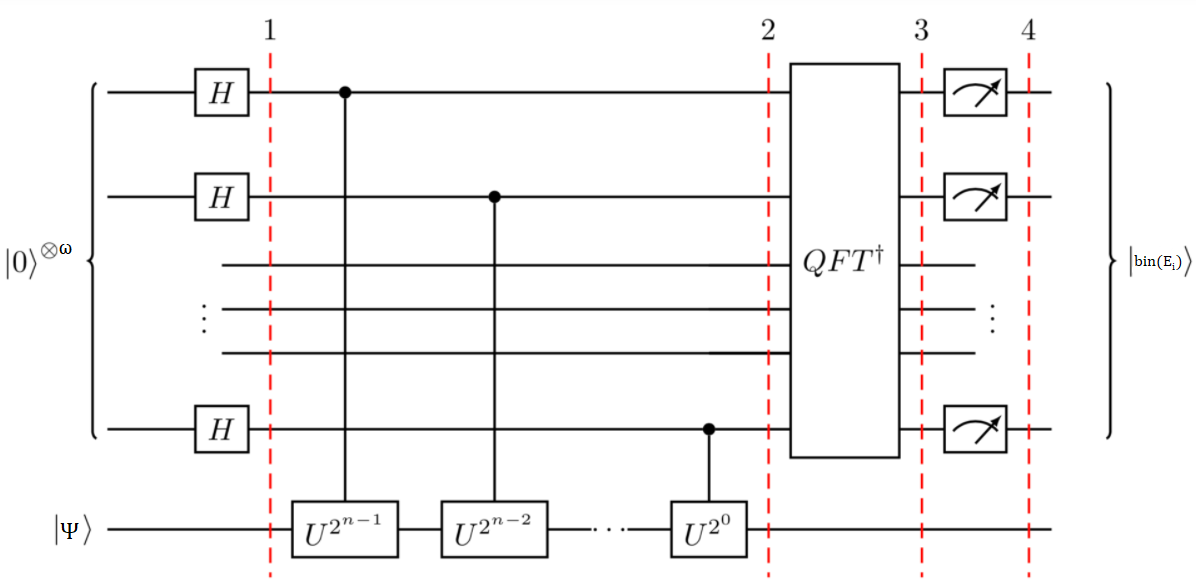
\includegraphics[width=0.95\textwidth]{figures/Phase estimation circuit.png}
  \caption{Circuital scheme of the QPE algorithm.} \label{QPE}
\end{figure} \\
In the following we analyze the two main components of the QPE method: the state preparation and the implementation of the controlled-$U^{2^j}$ operation.

\subsection{State preparation}
Initializing the qubit register in a state which has a sufficiently large overlap with the target eigenstate, typically the ground state, is a nontrivial problem. This is important because a randomly chosen state would have an exponentially vanishing probability of collapsing to the desired ground state as the system size increases. This highlights the necessity of developing state preparation routines which result in, at worst, a polynomially decreasing overlap with the FCI ground state as the system size increases. \\
Several techniques have been proposed for state preparation. One approach is to prepare reference states obtained from classically tractable calculations. Alternatively, we can use the variational methods discussed in Chapter \ref{Quantum computing for computational chemistry: NISQ devices}. \\
\\
Another method is adiabatic state preparation (ASP), an approach inspired by the adiabatic model of quantum computation. To do so, we first start with a simple Hamiltonian $H_0$ and prepare its ground state. We then time evolve the system under a Hamiltonian that changes slowly from $H_0$ to $H_s$, thus preparing a state that is close to the ground state of $H_s$. The efficiency of ASP  depends on the gap between the ground state and the first excited state along the path between $H_0$ and $H_s$. For chemical systems, ASP may be achieved by initializing the system in the ground state of the Hartree-Fock Hamiltonian ($H_0$), and interpolating between the initial and final Hamiltonians using an annealing schedule such as $H(t) = (1-t/T)H_0 + (t/T)H_s$, where $t$ is the time and $T$ is the the maximum desired simulation time \cite{McArdle2020Mar}. \\
Numerical simulations support this method, it was shown that annealing times for methylene (CH$_2$) could be reduced by up to 4 orders of magnitude by using an initial state with larger overlap with the true ground state \cite{Veis2014Jun}. We note, however, that if an initial state with sufficiently large overlap with the ground state is available, we may be able to forgo ASP entirely and instead carry out phase estimation directly on that initial state. As discussed previously, phase estimation requires only a non-negligible overlap with the target ground state.

\subsection{Hamiltonian simulation}
As discussed, the canonical phase estimation algorithm require implementation of the time evolution operator $e^{-iHt}$, where $H$ may or may be not time dependent. As described in Chapter \ref{Quantum computing}, the simulation of Hamiltonian dynamics, i.e. the solution of the time-dependent Schrödinger equation (TDSE), is a $\bf{BQP}$-complete problem, and thus a natural application for a quantum computer \cite{Motta2021Dec}. \\
There are several ways to do this, each with its own advantages and disadvantages. \\
The most simple method for time evolution is the Trotter decomposition formula, which we have used here to describe the algorithm. If a time-independent Hamiltonian $H$ can be decomposed as $H = \sum_i h_i$, where $h_i$ are local Hamiltonians, then a first order Lie-Trotter-Suzuki approximation of the time evolution is
\begin{equation}
    U = e^{-iHt} = e^{-i\sum_i h_i t} = \left( \prod_i e^{-i h_i t/S} \right)^S + O(t^2 / S),
\end{equation}
This approach is also referred to as the 'product formula' method. In practice, to achieve accuracy $\epsilon$ in the retrieving of the correct unitary evolution, the number of Trotter steps $S = O(t^2/\epsilon)$ should be large in order to suppress the errors in the approximation. This is effectively a step by step evolution under time evolution operators corresponding to each of the terms in the Hamiltonian. It is also possible to use higher order product formulas, which scale better with respect to the simulation error than the first order method. Randomization procedures, such as randomly ordering the terms in the Trotter sequence or stochastically choosing which terms to include in the Hamiltonian, have been shown to improve the accuracy obtained using product formulas. \\
Product formulas can also be used to simulate dynamics under a time-dependent Hamiltonian $H(t)$ and it can be shown that the accuracy of such simulations depends on the derivatives of the Hamiltonian \cite{Wiebe2011Oct}. \\
\\
Alternative methods that may realize the time evolution operator more efficiently than Trotterization have been introduced, including quantum-walk-based methods, multiproduct formulas and qubitization. One approach is the 'linear combinations of unitaries' (LCU) query model, which decomposes the Hamiltonian or time evolution operator into a linear combination of unitary operators that are then applied in superposition using oracle circuits. These must be explicitly constructed for a given problem. \\
As a linear combination of unitaries is itself not necessarily unitary, these approaches may require additional techniques such as amplitude amplification to maintain a high probability of success \cite{Motta2021Dec}.

\section{Computational requirements}
A complete analysis of the computational requirements for quantum algorithms is hard to achieve, since it highly depends on the device architecture and the target of the simulation, but we can study some common indicators in order to do a comparison between different methods. \\
The algorithmic parameters that we consider here are:
\begin{itemize}
    \item \textbf{Circuit width ($n_q$)} \\
    i.e. the number of qubits in the registers;
    
    \item \textbf{Circuit depth ($n_g$)} \\
    i.e. the number of layers of gates that must be applied, where a layer of gates is a set of gates that can be applied simultaneously;
    
    \item \textbf{Repetitions ($n_{rep}$)} \\
    i.e. the number of times the circuit must be performed, but not the measurement, to obtain the result;
    
    \item \textbf{Total scaling ($n_t = n_g \cdot n_{rep}$)}.
\end{itemize}
In Chapter \ref{Computational advantage} we will also refer to technological inspired characteristics like connectivity or coherence time. \\
\\
Generally speaking the depth and the repetitions for the QPE algorithm scale as
\begin{equation}
    n_g = O\left(\frac{1}{\epsilon}\right), \ n_{rep} = O(1),
\end{equation}
where $\epsilon$ is the error between the result and the correct value of the phase $\varphi$, or equivalently the accuracy of the estimate of the algorithm. \\
If we consider the simulation of a quantum system ($\varphi = E_i$), then we have to consider: first, the probability overlap $\eta$ of the initial state with the target state $\ket{\chi_i}$; second, depending on the method used to do the simulation, the coefficients of the resulting qubit Hamiltonian, which can be summarized with the limit value $E_{max} = \sum_i |w_i|$; finally the number of orbitals, $m$, with which we model the electrons. Thus the circuit depth scales as
\begin{equation}
    n_g = O\left(\frac{E_{max} m}{\epsilon \eta}\right).
\end{equation}
As for the width, QPE requires approximately $m$ qubits to store the relevant quantum state,
\begin{equation}
    n_q = O(m).
\end{equation}
However, QPE typically also requires additional auxiliary qubits. \\
First, such qubits are needed to store the bits corresponding to the numerical value of the energy estimate. The number of ancilla qubits $\omega$ required is determined by the desired success probability and precision. If the phase $E_i$ can not be written exactly with a $\omega$ binary expression, one can prove that to successfully obtain $E_i$ accurate to $n$ bits with probability of success at least $1 - \epsilon$ we choose \cite{Nielsen2010Dec}
\begin{equation}
    \omega = n + \biggl\lceil log \left( 2 + \frac{1}{2\epsilon} \right) \biggr\rceil,
\end{equation}
however, this can be reduced to just a single qubit using iterative phase estimation. \\
Auxiliary qubits are also required for some methods of implementing the required unitary operators, but this is negligible for the most recent methods. \\
Secondly, since the circuits used when performing QPE are very deep we expect error correction procedures to be required in order to obtain useful results from the calculations. This introduce an overhead on both the circuit width (spatial overhead) and depth (temporal overhead). We write these overheads as $\theta_S$ and $\theta_T$ respectively. \\
For the surface code, which is one of the most researched, the overheads are determined by the code distance, $d$, with $\theta_S \sim d^2$ and $\theta_T \sim d$, and therefore $\theta_S \sim \theta_T^2$. We note that, in order to maintain a constant probability of a logical error occurring, these overheads must increase with increasing logical circuit depth and number of logical qubits; however, they increase logarithmically and so we ignore this here.
In conclusion, the algorithmic parameters scale as \cite{Blunt2022Jun}
\begin{equation}
    n_q^{QPE} = O(m \theta_T^2), \ n_g^{QPE} = O\left( \frac{E_{max} m \theta_T}{\epsilon \eta} \right), \ n_{rep}^{QPE} = O\left( \frac{1}{\eta} \right). \label{Scaling QPE}
\end{equation}
In the next chapter we will see how these parameters, especially the number of measurements, are related to the coefficients in the qubit Hamiltonian. For now we use the result from Lee et al. \cite{Lee2020Nov}, which states that $E_{max}$ scales between $O(m)$ and $O(m^3)$. \\
Thus the total scaling of the QPE algorithm is
\begin{equation}
    n_t^{QPE} = n_g^{QPE} \cdot n_{rep}^{QPE} = O\left( \frac{E_{max} m \theta_T}{\epsilon \eta^2} \right). \label{Scaling QPE 1}
\end{equation}

\subsection{Examples}
Several studies estimated the resource requirements for QPE methods by combining and comparing different components of the algorithm and the general consensus is that the fault-tolerant overhead and the long coherence time needed to execute the algorithm make the method very expensive, but at the same time the most accurate one can use for simulation. We discuss more on this in Chapter \ref{Computational advantage}. \\
\\
One of the first estimates for the QPE algorithm applied to molecular systems was made by Alan Aspuru-Guzik et al. in 2005 \cite{Aspuru-Guzik2005Sep}. They showed that the number of qubits required for both the compact and direct mappings scales linearly with the number of basis functions. For the compact mapping the qubit requirement depends also on the ratio of number of electrons to basis functions, which is relatively constant for a given basis set. \\
Although the higher quality cc-pVTZ basis is more economical per basis function, a molecule in this basis uses substantially more functions than with the 6-31G* basis. This trend and the qubits required for specific molecules and basis sets are represented in Figure \ref{Aspuru-Guzik}. \\
\begin{figure}[ht]
  \centering
  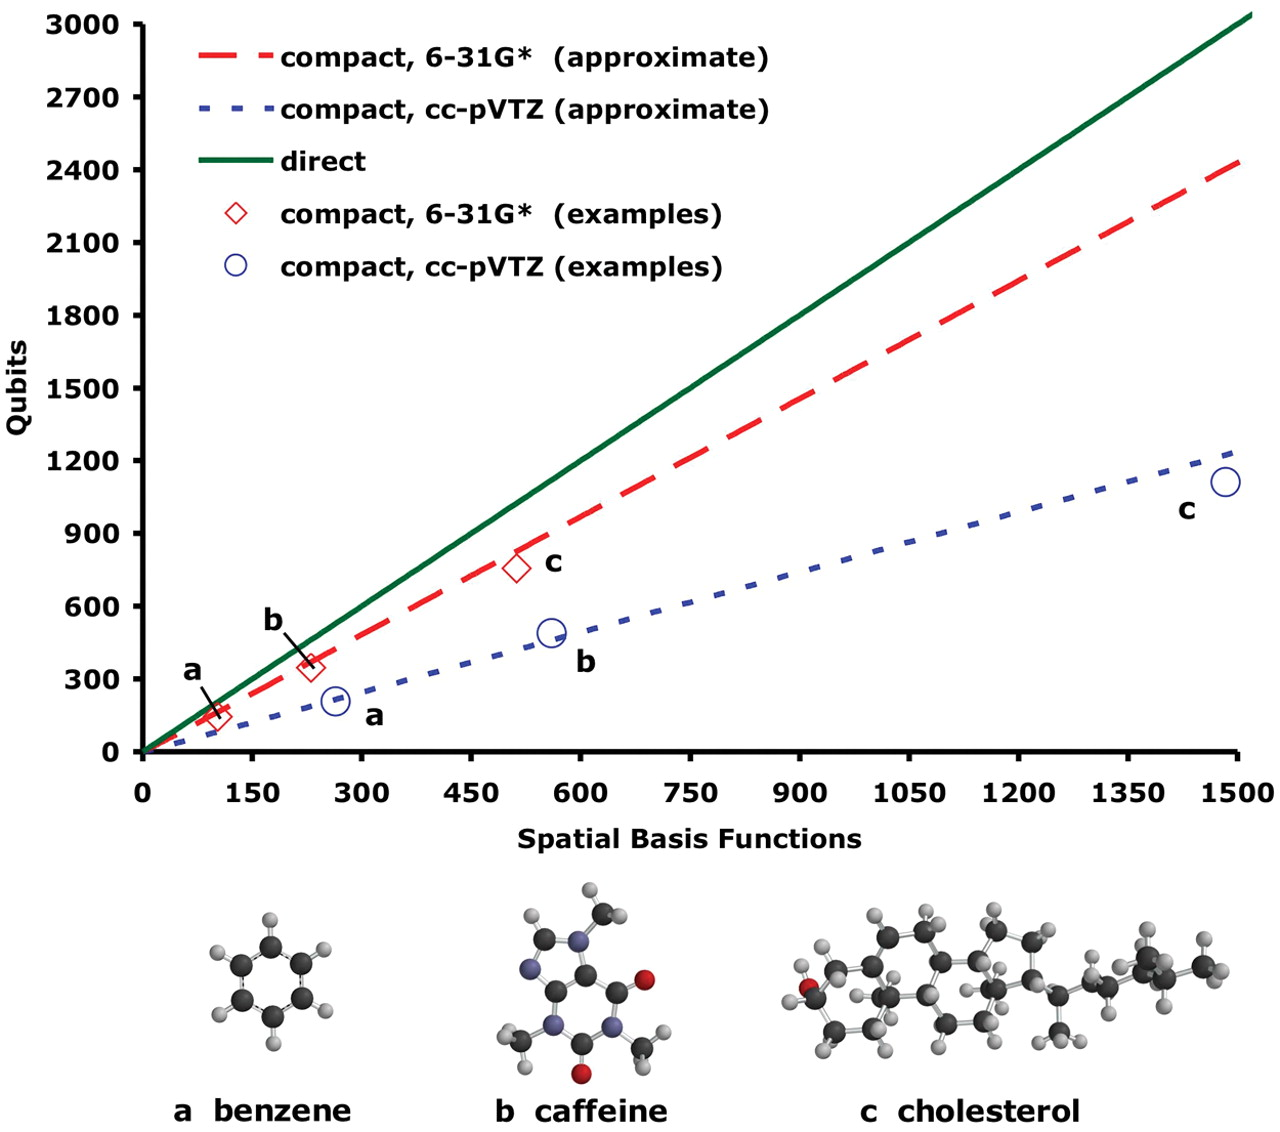
\includegraphics[width=0.8\textwidth]{figures/Aspuru-Guzik.jpeg}
  \caption{Qubit requirements versus basis size \cite{Aspuru-Guzik2005Sep}.} \label{Aspuru-Guzik}
\end{figure} \\
In this research they carried out calculations on H$_2$O and LiH. For the former they used the minimal STO-3G basis set, yielding 196 singlet-spin configurations, and for the latter they used the larger 6-31G basis yielding 1210 such configurations. The algorithm they used is a modified QPE which uses a relatively small number of qubits. The sequence is: a reference energy is estimated, then the Hamiltonian in shifted by that value and an estimate of the deviation is computed, then the reference energy is updated and the procedure is repeated until the desired precision is obtained. With each iteration one additional bit of $E$ is obtained. \\
After 20 iterations the electronic energy obtained for H$_2$O matched the Hamiltonian diagonalization energy and so did the LiH calculation, both within chemical accuracy. \\
They ended up proving that the lengths of the gate sequences involved are bounded from above by a polynomial function of the number of qubits. This a consequence of the decomposition of the unitary evolution operator. \\
Moreover, analyzing the mappings between fermionic and qubit Hamiltonians we will see that the number of terms grows approximately with the fourth power of the number of orbitals, thus, the most expensive part would be the the number of one- and two-qubits elementary gates used to represent an arbitrary four-qubit unitary operation. \\
\\
A more recent estimate on the QPE algorithm has been presented by Markus Reiher et al. in 2017 \cite{Reiher2017Jul}. They considered the chemical process of biological nitrogen fixation by the enzyme nitrogenase, also called MoFe protein. This enzyme accomplishes the remarkable transformation of turning a dinitrogen molecule into two ammonia molecules and one dihydrogen molecule under ambient conditions. Whereas the industrial Haber-Bosch catalyst requires high temperatures and pressures and is therefore energy intensive, the active site of Modependent nitrogenase (the iron molybdenum cofactor or FeMoco) can split the dinitrogen triple bond at room temperature and standard pressure. Mo-dependent nitrogenase consists of two subunits, the Fe protein, a homodimer, and the MoFe protein, an $\alpha_2 \beta_2$ tetramer. Its X-ray crystal structure is shown in Figure \ref{MoFe and FeMoco}. \\
Despite the importance of this process for fertilizer production that makes nitrogen from air accessible to plants, the mechanism of nitrogen fixation at FeMoco is not yet completely understood. \\
\begin{figure}[ht]
  \centering
  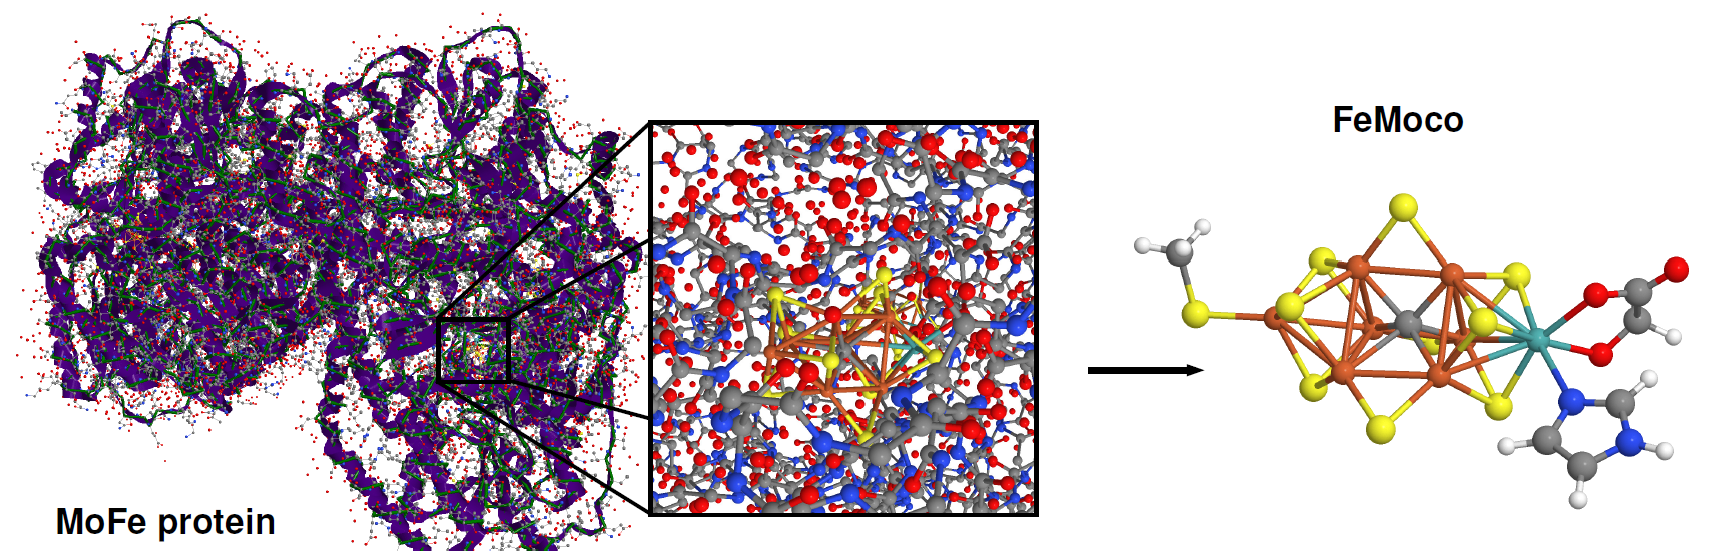
\includegraphics[width=\textwidth]{figures/MoFe and FeMoco.png}
  \caption{Structure of the MoFe protein and the FeMoco active site \cite{Reiher2017Jul}.} \label{MoFe and FeMoco}
\end{figure} \\
Authors used standard DFT, with B3LYP functional, for molecular structure optimization, thanks to its low computational requirements even for complex many-body systems like this one, and studied the active site with a quantum computer that accesses truly large active orbital spaces, the latter is sometimes called multi-configuration wave function model or complete active space (CAS) method, if all the combinations of the active space orbitals are included. They focused on QPE using the Trotter decomposition formula. \\
In order to consider error correction in the algorithm they made two approximations. \\
First, the exponentials in the Trotter formula are decomposed into single-qubit rotations and Clifford gates. In the surface code, which they considered for qubit encodings, Clifford gates can be implemented fault tolerantly; the single-qubit rotations, however, require approximation by a discrete set of gates consisting of Clifford operations and at least one non-Clifford operation, usually taken to be the $T$ gate, a rotation by $\pi/8$ about the z-axis. Each $T$ gate requires a procedure called 'magic state distillation', which consumes a host of noisy quantum states to output a single accurate magic state. \\
Secondly, the magic state is used to teleport a $T$ gate into the computation. \\
The space and time overheads of state distillation render it by far the most costly aspect of quantum error correction, leading to a large multiplicative overhead for each single-qubit rotation. The number of $T$ gates therefore typically dominates the cost when implementing a fault tolerant algorithm. \\
\\
The resource estimates are based on extrapolations from the costs found from simulations of smaller molecules and focus on two protoypical structures of FeMoco, one with 54 electrons in 54 spatial orbitals (108 spin-orbitals) and the second with 65 electrons and 57 spatial (114 spin-orbitals) orbitals. Moreover, the calculation is conducted within a basis set that is a reasonable match for the target accuracy required on the energy value, i.e. 1 mHa (chemical accuracy) and 0.1 mHa. These errors include the error in phase estimation, the error in the Trotter deocomposition and errors from decomposing the Trotter approximation into $H$ and $T$ gates. \\
Three implementations of the quantum algorithm are considered. Serial: the single-qubit rotations are constrained to occur serially. Nesting approach: Hamiltonian terms that affect disjoint sets of spin-orbitals are executed in parallel, which substantially reduces the runtime of the calculations. Programmable ancilla rotations (PAR), rotations are cached in qubits, which are then teleported into the circuit as needed. \\
The cost in terms of logical qubits is shown in Figure \ref{FeMoco - table 1}.
\begin{figure}[ht]
  \centering
  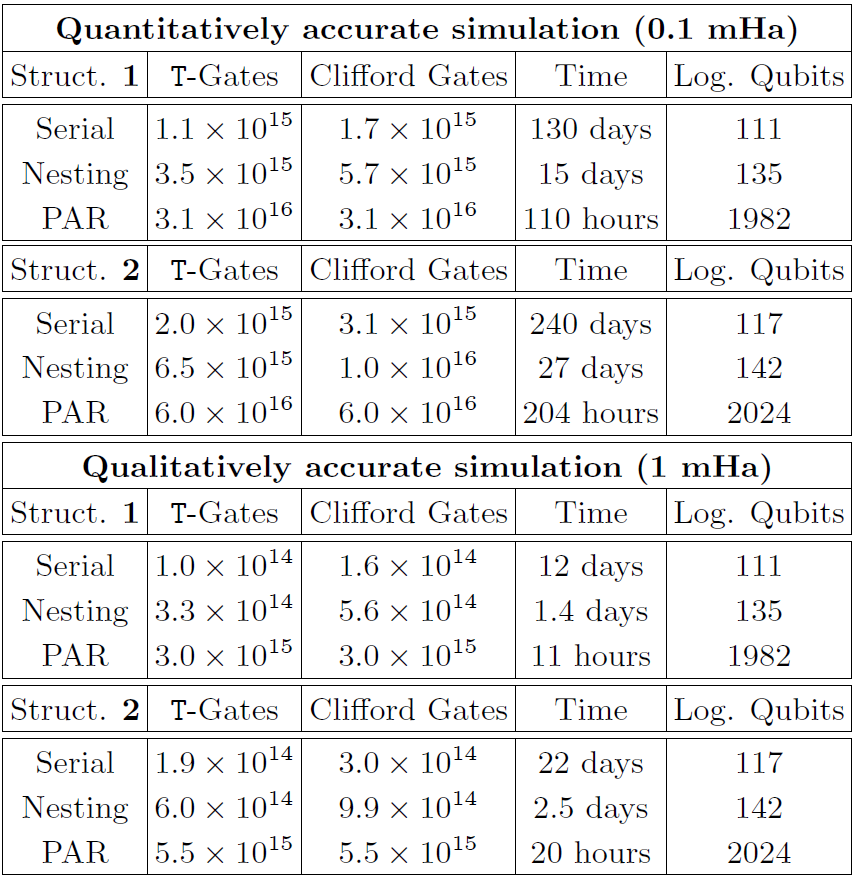
\includegraphics[width=0.65\textwidth]{figures/FeMoco - table 1.png}
  \caption{Simulation time and resources estimate for FeMoco \cite{Reiher2017Jul}.} \label{FeMoco - table 1}
\end{figure} \\
We can see that the nesting approach gives a reasonably trade-off between the other methods. \\
To complete the resource estimate the authors added the overheads required to perform the simulation fault tolerantly. The physical error rates in the hardware is assumed to be: $10^{-3}$, a near-term standard, $10^{-6}$ or $10^{-9}$, which might be achieved in future. The results are shown in Figure \ref{FeMoco - table 2}.
\begin{figure}[ht]
  \centering
  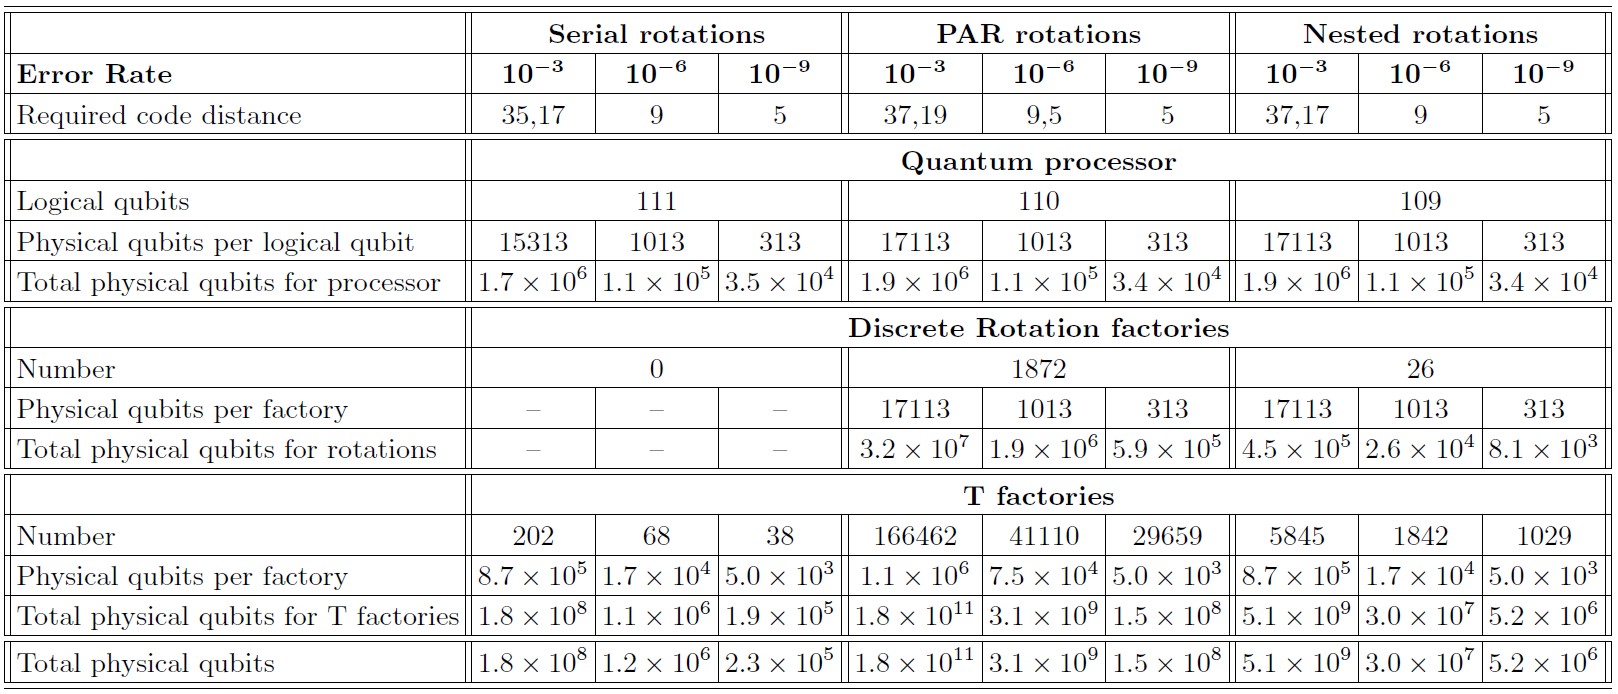
\includegraphics[width=\textwidth]{figures/FeMoco - table 2.png}
  \caption{Resource estimates including error correction \cite{Reiher2017Jul}.} \label{FeMoco - table 2}
\end{figure} \\
The number of logical qubits in the main quantum processor is in the hundreds, which translates into tens of thousands up to millions of physical qubits. Most of the qubits are used in the $T$ factories, each of which needs fewer physical qubits than the main quantum processor. \\
The authors also noted that the required quantum computing resources are comparable to that needed for Shor's factoring algorithm for interesting 4096 bit numbers, both in terms of number of gates and also physical qubits. Also, the resources required depend sensitively on gate error rates.